\PassOptionsToPackage{dvipsnames}{xcolor}

\documentclass{article}
\usepackage[margin=1.2in]{geometry}
\usepackage[T1]{fontenc}
\usepackage[backend=bibtex8]{biblatex}
\usepackage{tikz,xspace,xstring,amsmath,amssymb,beramono,multirow,graphicx}
\usepackage{lmodern}
\usepackage{listings}% http://ctan.org/pkg/listings
\usepackage{xcolor}% http://ctan.org/pkg/xcolor
\addbibresource{references.bib}
\usetikzlibrary{shapes,arrows,matrix,calc}

\tikzset{table matrix/.style={draw=black,thick,inner sep=0,fill=white,matrix of nodes, nodes in empty cells,%
nodes={minimum width=45mm,minimum height=3mm,draw,outer sep=0,inner sep=0},
      }
}


% hackery from http://tex.stackexchange.com/questions/15237/highlight-text-in-code-listing-while-also-keeping-syntax-highlighting
\makeatletter
\newenvironment{btHighlight}[1][]
{\begingroup\tikzset{bt@Highlight@par/.style={#1}}\begin{lrbox}{\@tempboxa}}
{\end{lrbox}\bt@HL@box[bt@Highlight@par]{\@tempboxa}\endgroup}

\newcommand\btHL[1][]{%
  \begin{btHighlight}[#1]\bgroup\aftergroup\bt@HL@endenv%
}
\def\bt@HL@endenv{%
  \end{btHighlight}%   
  \egroup
}
\newcommand{\bt@HL@box}[2][]{%
  \tikz[#1]{%
    \pgfpathrectangle{\pgfpoint{1pt}{0pt}}{\pgfpoint{\wd #2}{\ht #2}}%
    \pgfusepath{use as bounding box}%
    \node[anchor=base west, fill=orange!30,outer sep=0pt,inner xsep=1pt, inner ysep=0pt, rounded corners=3pt, minimum height=\ht\strutbox+1pt,#1]{\raisebox{1pt}{\strut}\strut\usebox{#2}};
  }%
}
\makeatother


\definecolor{bluekeywords}{rgb}{0.13,0.13,1}
\definecolor{greencomments}{rgb}{0,0.5,0}
\definecolor{turqusnumbers}{rgb}{0.17,0.57,0.69}
\definecolor{redstrings}{rgb}{0.5,0,0}

\newcommand{\bt}{\ensuremath{^{\backprime}}}

\lstdefinelanguage{FSharp}
    {morekeywords={let, new, match, with, rec, open, module, namespace, type, of, member, and, for, in, do, begin, end, fun, function, try, mutable, if, then, else},
    keywordstyle=\color{bluekeywords},
    sensitive=true,
    morecomment=[l][\color{greencomments}]{///},
    morecomment=[l][\color{greencomments}]{//},
    morecomment=[s][\color{greencomments}]{{(*}{*)}},
    morestring=[b]",
    stringstyle=\color{redstrings}
    }

\lstnewenvironment{fslisting}
  {
    \lstset{
        language=FSharp,
        basicstyle=\ttfamily,
        breaklines=true,
        columns=fullflexible,
		tabsize=4
     }
  }
  {
  }

\lstdefinelanguage{soop} {
	morekeywords={using, namespace, class, struct, interface, mixin, if, then, else, while, for, this, var, val, static, private, public, where, true, false, return},
	keywordstyle=\color{bluekeywords},
	sensitive=true,
	morecomment=[l][\color{greencomments}]{//},
	morecomment=[s][\color{greencomments}]{{/*}{*/}},
	morestring=[b]",
    stringstyle=\color{redstrings}
}

\lstnewenvironment{sooplisting}
  {
    \lstset{
        language=soop,
        basicstyle=\ttfamily,
        breaklines=true,
        columns=fullflexible,
		tabsize=4,
        literate={`}{{\bt}}1 {...}{{\ensuremath{\dots}}}1,
        moredelim=**[is][{\btHL[fill=green!20]}]{~~}{~~}
      }
  }
  {
  }
  
\lstnewenvironment{javalisting}
  {
     \lstset{
        language=Java,
        keywordstyle=\color{bluekeywords},
        commentstyle=\color{greencomments},
        basicstyle=\ttfamily,
        breaklines=true,
        columns=fullflexible,
		tabsize=4,
        literate={`}{{\bt}}1 {...}{{\ensuremath{\dots}}}1
     }
  }{}

\lstdefinelanguage{llvm}{
  morecomment = [l]{;},
  morestring=[b]", 
  sensitive = true,
  classoffset=0,
  morekeywords={
    define, declare, global, constant,
    internal, external, private,
    linkonce, linkonce_odr, weak, weak_odr, appending,
    common, extern_weak,
    thread_local, dllimport, dllexport,
    hidden, protected, default,
    except, deplibs,
    volatile, fastcc, coldcc, cc, ccc,
    x86_stdcallcc, x86_fastcallcc,
    ptx_kernel, ptx_device,
    signext, zeroext, inreg, sret, nounwind, noreturn,
    nocapture, byval, nest, readnone, readonly, noalias, uwtable,
    inlinehint, noinline, alwaysinline, optsize, ssp, sspreq,
    noredzone, noimplicitfloat, naked, alignstack,
    module, asm, align, tail, to,
    addrspace, section, alias, sideeffect, c, gc,
    target, datalayout, triple,
    blockaddress
  },
  classoffset=1, keywordstyle=\color{purple},
  morekeywords={
    fadd, sub, fsub, mul, fmul,
    sdiv, udiv, fdiv, srem, urem, frem,
    and, or, xor,
    icmp, fcmp,
    eq, ne, ugt, uge, ult, ule, sgt, sge, slt, sle,
    oeq, ogt, oge, olt, ole, one, ord, ueq, ugt, uge,
    ult, ule, une, uno,
    nuw, nsw, exact, inbounds,
    phi, call, select, shl, lshr, ashr, va_arg,
    trunc, zext, sext,
    fptrunc, fpext, fptoui, fptosi, uitofp, sitofp,
    ptrtoint, inttoptr, bitcast,
    ret, br, indirectbr, switch, invoke, unwind, unreachable,
    malloc, alloca, free, load, store, getelementptr,
    extractelement, insertelement, shufflevector,
    extractvalue, insertvalue,
  },
  alsoletter={\%},
  keywordsprefix={\%},
}

\lstnewenvironment{llvmlisting}
  {
    \lstset{
        language=llvm,
        basicstyle=\ttfamily,
        breaklines=true,
        columns=fullflexible,
        keywordstyle=\ttfamily\color[rgb]{0,0,1},
    	commentstyle=\ttfamily\color[rgb]{0.133,0.545,0.133},
   		stringstyle=\ttfamily\color[rgb]{0.627,0.126,0.941}
  	}
  }
  {
  }

\newcommand{\sharponend}[1]{{\settoheight{\dimen0}{#1}#1\kern-.05em \resizebox{!}{\dimen0}{\raisebox{\depth}{\fontseries{b}\selectfont\#}}}}

\newcommand{\fsharp}{\sharponend{F}\xspace}
\newcommand{\csharp}{\sharponend{C}\xspace}
\newcommand*{\cpp}{C\ensuremath{++}\xspace}

\newcommand{\code}[1]{\texttt{\StrSubstitute{#1}{`}{\bt}}}
\newcommand{\bcode}[1]{\code{#1}}

\newcommand{\codelst}[1]{\\\>#1\\}

\newcommand{\plname}[0]{Drake\xspace}

\tikzstyle{block} = [rectangle, draw, fill=blue!20, 
    text width=5em, text centered, rounded corners, minimum height=4em]
\tikzstyle{line} = [draw, -latex']


\begin{document}
\title{An Object Oriented Compiler}
\author{Callum Rogers}
\maketitle

\begin{abstract}
This project report describes the design and implementation of a compiler for a statically typed, memory safe, object oriented programming language called \plname. It explores the problems of code reuse, mutability and (lack of) null saftey that occurs in other statically typed object oriented programming languages and presents solutions (with implementations) to these problems. A detailed account of the architecture of the compiler, it's implementation and various problems that were encountered along the way follows, with explorations of different possible implementations and explanations as to why they were not chosen.
\end{abstract}

\pagebreak
\tableofcontents
\pagebreak

\section{Introduction}
We will first explore the history and core features of object oriented programming, followed by some motivations for taking this project which stem from issues encountered when using other object oriented programming languages.

\subsection{Brief Introduction to Object Oriented Programming}
\label{sec:OOPIntro}
In the last 50 years object oriented programming languages have risen to become the most popular programming paradigm with languages such as Java, \cpp and \csharp being the most searched and most widely used\cite{TIOBE}. Object Oriented Programming (OOP) comprises of \textit{objects} that have \textit{data-fields} -- the state which describes the object; and \textit{methods} -- procedures that are associated with a particular instance of an object. \textit{B. Pierce} in 2000 came up with a good core set of features that an object oriented programming language should implement\cite[p.~225-227]{PIERCE:2002}:
\begin{enumerate}
	\item{\textbf{Polymorphism.} When a method is invoked on an object, the state of the object determines which code is executed. Two objects with the same set of methods (i.e. with the same \textit{interface}) may have different implementations and choosing which implementation to execute at run time involves looking up the method's name in a \textit{method table} that is attached to each object (\textit{dynamic dispatch}).}
	\item{\textbf{Encapsulation.} Much of the internal state of the object is hidden and can be accessed or modified by the classes own methods. When the internal representation of an object changes, only a small region of the entire program is affected, greatly improving the program's maintainability.} 
	\item{\textbf{Subtyping.} The type of an object is defined by its operations -- the set of it's methods and fields. If an object $A$ implements a subset of the operations of an object $B$ any context expecting an $A$ object can be given a $B$ object.}
	\item{\textbf{Behavioural Reuse.} Objects that share similar interfaces may also want to share similar behaviours -- there should be a way to define a behaviour in one place but use it for many objects (code reuse).}
\end{enumerate}

\subsection{Motivation}
In many statically typed object oriented programming languages code reuse is usually limited in a number of ways; generally, you have the option of using inheritance or composition and delegation to reuse code. However, the use of inheritance carries with it a large number of issues and techniques to solve the same problem using composition and delegation in languages such as Java, \csharp and \cpp can lead to unmanageable amounts of boilerplate code which is hard to maintain.

\subsubsection{Problems with Inheritance For Code Reuse}
Inheritance for classes in object oriented languages can come in two flavours: \textit{single inheritance}, where a class inherits from one superclass, and \textit{multiple inheritance}, where a class can inherit from multiple superclasses. Both of these approaches have disadvantages when trying to use inheritance for code reuse.

\paragraph{Common Issues.}
\label{sec:CommonIssuesInheritance}
Inheritance in general causes problems of tight coupling and loss of flexibility. When a class inherits from a superclass it has to implement a very strong ``is-a'' relation that requires the class to implement all of the public methods of the superclass. This does not allow the class to select a subset of the public interface of the superclass and means that extra methods that do not fit in the requirements can appear. The classic real world example of this is the \bcode{Stack<E>}\cite{JavaStack} class in the Java standard library that inherits from \bcode{Vector<E>}, which means the method \bcode{insertElementAt(E,int)} is inherited from \bcode{Vector<E>} that can be used to break the last-in-last-out semantics expected in a stack.

\paragraph{Single Inheritance.}
The largest problem with single inheritance is that it restricts a class to having only a single superclass; this means some relationships cannot be modelled. For example, we can have a class \bcode{Vehicle} that contains a vehicle's speed and mileage and a class \bcode{Asset} that contains the asset's value. A \bcode{Car} is both a \bcode{Vehicle} \textit{and} an \bcode{Asset} but we are limited to making a \bcode{Car} either a \bcode{Vehicle} \textit{or} an \bcode{Asset}.

\paragraph{Multiple Inheritance.}
Multiple inheritance provides much greater flexibility than single inheritance but bring with it a bevy of problems. The main issue is the ``Diamond Problem'', where a class inherits from two superclasses that each inherit from another superclass. In the case of the \bcode{Car/Vehicle/Asset} example, both \bcode{Vehicle} and \bcode{Asset} inherit from \bcode{Object} which has the method \bcode{toString()}. If \bcode{toString()} is overridden in both \bcode{Vehicle} and \bcode{Asset}, for the expression \bcode{car.toString()} the compiler now has to decide between using the method inherited from \bcode{Vehicle} and \bcode{Asset}.

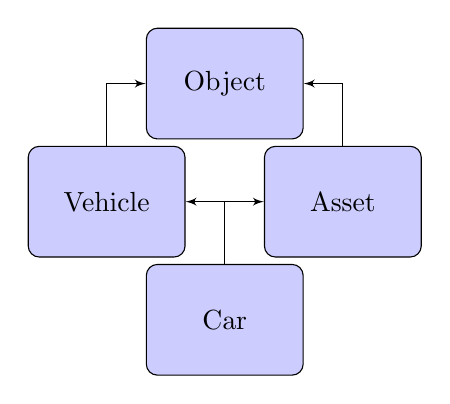
\begin{tikzpicture}
	\node [block] (D) at (3,0) {Car};
	\node [block] (B) at (1.5,1.5) {Vehicle};
	\node [block] (C) at (4.5,1.5) {Asset};
	\node [block] (A) at (3,3) {Object};
	
	\path [line] (D) |- (B);
	\path [line] (D) |- (C);
	\path [line] (B) |- (A);
	\path [line] (C) |- (A);
\end{tikzpicture}

\paragraph{Composition and Delegation}
\label{sec:CompAndDel}
Every case of inheritance can be re-modelled using only \textit{composition} (building up objects from other objects) and \textit{delegation} (passing on a task to another piece of the program). Instead of inheriting from superclasses, we include an instance of the `superclass' as a field in our class (\textit{composition}) and select which of it's public methods we want to expose in the class' public interface by creating \textit{forwarding methods} which pass off the task to the `superclass' instance (\textit{delegation}).

This allows the class to have multiple units of code reuse as it can instantiate as many `superclasses' as it needs and greater flexibility as there is the choice not to include all the public methods present in the `superclass'. The Diamond Problem is no longer and issue as the naming in resolved in each class by the forwarding methods. An added bonus is that we can perform \textit{dynamic binding} by changing the instance of the `superclass' to one that has a different behaviour. The `superclass' implements an interface that means that any other concrete behaviour can be constructed if needed. The following example of Java code implements the \bcode{Car/Vehicle/Asset} example:
\begin{javalisting}
interface Vehicle {
	double speed();
	double mileage();
}

interface Asset {
	long value();
}

class VehicleImpl implements Vehicle {...}

class AssetImpl implements Asset {...}

class Car implements Vehicle, Asset {
	// Composition
	private Vehicle vehicle = new VehicleImpl();
	private Asset asset = new AssetImpl();

	// Delegation/Forwarding Methods
	public double speed() { return vehicle.speed(); }
	public double mileage() { return vehicle.mileage(); }
	public long value() { return asset.value(); }
}
\end{javalisting}
The problem with this approach, however, is that 

\subsubsection{Null safety}
Tony Hoare described his invention of the null reference for the type system of ALGOL in 1965 as his ``billion-dollar mistake'' due to ``innumerable errors, vulnerabilities, and system crashes'' that have occurred due to it's use\cite{HOARE:2009}. Conceptually, references are a form of indirection that we can follow to access some resource. A nullable reference is \textit{either} an indirection to access some resource \textit{or} an indication that there is no resource. In languages where all references are nullable (Java, \csharp, \cpp), in the cases where variables are expected to always have a reference to a resource there always exists the possibility that it could be \bcode{null}, meaning that accessing it requires \bcode{null} checks and appropriate error handling or accepting that it could cause an error when it dereferences.

\subsubsection{Mutability by default}
Most other OOP languages assume mutability of variables by default -- this is a problem as the easiest thing for the programmer to do is not use extra keywords like \bcode{final} in Java but just leave the variable declarations mutable as is even when they should not change. This allows subtle bugs to creep in, especially for large systems, where a certain variable is set to another value even when it should not be and the proliferation of mutability makes it harder to reason about programs.

\subsection{Aims}
The aims of this project were to build a compiler from the ground up with the following features:
\begin{itemize}
	\item{Statically typed, memory safe and object oriented.}
	\item{Has a solution to the problems of code reuse through inheritance, null safety and mutability by default listed above.}
	\item{Has some form of parametric polymorphism, so that types can handle many different data types without depending on their type and so increase the expressiveness of the language.}
	\item{Is reasonably fast, of comparable speed to similar languages such as Java and \csharp.}
\end{itemize}

\subsection{Structure of Report}
First, a brief introduction to the major and interesting features of the \plname programming language, explaining the syntax and the semantics of the language as well as how it fulfils the aims of the project. Then an overview of the architecture of the implementation -- how the project is technically constructed, how it was tested, which technologies were used to build it -- as well as some background information required to understand the following sections. Thirdly, an in-depth look at how the language features are implemented in the compiler and their resulting output with discussion about the merits and drawbacks of each possible implementation. Finally, a review of the entire project with difficulties and lessons learnt along the way and whether it has met it's aims, with a list of possible future work. 

\pagebreak
\section{An Introduction to \plname}
The syntax of \plname will be familiar to anyone who has worked with ``curly brace'' object oriented languages such as \cpp, Java and \csharp but with some important semantic differences. This section will describe the features of \plname one by one. To dive straight in and get a feel of the language, the program below recursively calculates the factorial of 6 and prints the result:
\begin{sooplisting}
using System;

namespace T {
	class Program {
		static fac(n: Int32): Int32 {
			if (n <= 1)
				return 1;
			return n * fac(n - 1);
		}

		public static main() {
			Console.println(fac(6));
		}
	}
}
\end{sooplisting}
\paragraph{Namespaces and Usings.}
A \bcode{namespace} is a module in which types are grouped together; this allow multiple types in different parts of the program to have the same name yet work independently of each other, similar to \csharp namespaces or Java packages. The \bcode{using X} statement allows all definitions in the file to access the types that exist in the namespace X. The \bcode{System} namespace contains most of the standard library for the \plname -- with types like integers, floats and arrays -- so is nearly always required. For brevity, every example following this will leave out the the \bcode{using} statements and \bcode{namespace} sections (it should be assumed there is a \bcode{using System;} statement included for every sample).
\\\\
A more extensive example is listed below; in this program, an array of \bcode{Calc} objects are created that perform different arithmetic operations via their \bcode{calc} method. These are then iterated over and have their operations applied to numbers, the results of which are then printed to the screen. The expected result is in the comment at the bottom and below that we analyse individual features of the language which make up this program.
\begin{sooplisting}
interface Calc {
	calc(i: Int32):Int23;
}

class Adder : Calc {
	private val amount = 0;

	public static new(amount: Int32):Adder {
		val add = ctor();
		add.amount = amount;
		return add;
	}

	public calc(i: Int32):Int32 { return i + amount; }
}

class Multiplier(private amount: Int32) : Calc {
	public calc(i: Int32): Int32 { return i * amount; }
}

class Program {
	static printMap(funcs: Array`[Calc]) {
		for (var i = 0; i < funcs.length(); i = i + 1) {
			val result = funcs[i].calc(i);
			Console.println(result);
		}
	}

	public static main() {
		val funcs = Array`[Calc].new(5);
		for (var i = 0; i < funcs.length(); i++) {
			if (i % 2 == 0)
				funcs[i] = [Calc] Adder.new(i);
			else
				funcs[i] = Multiplier.new(i);
		}
		printMap(funcs);
	}
}

/*[[[
0
1
4
9
8

]]]*/
\end{sooplisting}
\paragraph{Local Variables.}
\bcode{val} and \bcode{var} are used to define local and class variables -- \bcode{val} can only be assigned to once and so is immutable, \bcode{var} can be assigned to an unlimited number and is therefore mutable. Generally, \bcode{val} should be favoured where possible to prevent errors from modifying a reference when it should never have been modified. These constructs go some way to combat the ``Mutability by Default'' problem described in the previous section, as it is just as easy to write \bcode{val} as it is to write \bcode{var}.

\paragraph{Loops and Statements.}
If statements, while and for loops work as you would expect from similar languages like \csharp and Java.

\paragraph{Classes.}
Classes are the main way to make aggregate types in \plname; a class consists of a number of \textit{class variables} and \textit{class methods}. Class variables can be \textit{instance} variables (such as \bcode{Adder.amount}) where each object instantiation has its own variable instance, or \textit{static} variables where only one instance of each variable exists. Methods can either be \textit{instance} methods (such as \bcode{Adder.calc()}), which are called on an object and have access to it's state, or they are \textit{static} methods (such as \bcode{Program.printMap()}) that only have access to their parameters and other static methods/variables. \textit{Privacy modifiers} on a declaration allow the programmer to control which other code sections can access it -- \textit{private} means that only constructs within the current class can access the declaration where as \textit{public} means any construct in any part of the program can access it. If a privacy modifier is left out, the default is to set it to private. This allows encapsulation and the hiding of state from outside processes.

\paragraph{Constructors.}
A constructor is a public static method on a class $C$ that uses the inbuilt \bcode{ctor()} method -- \bcode{ctor()} returns an object of the type and size of $C$ where all the fields are zero initialised. In the example above, \bcode{Adder.new()} is a constructor. Every field must be initialised by the time the newly built object is returned and no field can be accessed before it is assigned to. An \textit{automatic constructor} (such as in \bcode{Multiplier}) can be used instead as a shorthand to writing an explicit constructor; code of this form:
\begin{sooplisting}
class Foo(x1: Type1, private x2: Type2, ..., public xN: TypeN) { /* decls */ }
\end{sooplisting}
is equivalent to code of the following form:
\begin{sooplisting}
class Foo {
	private val x1: Type1;
	private val x2: Type2;
	// ...
	public val xN: TypeN;
	
	public static new(x1: Type1, private x2: Type2, ..., public xN: TypeN) {
		var @ret = ctor();
		@ret.x1 = x1;
		@ret.x2 = x2;
		// ...
		@ret.xN = xN;
		return @ret;
	}
	
	/* decls */
}
\end{sooplisting}

\paragraph{Interfaces.}
Interfaces provide \textit{subtype polymorphism}; an interface defines a set of methods signatures that classes can implement and these classes can all be viewed as subtypes of the interface. This allows for \textit{dynamic dispatch} where the implementation of a method is decided at runtime by the type of the object the method is called on. In the example above, \bcode{Adder} and \bcode{Multiplier} both implement the \bcode{Calc} interface which provides the method \bcode{calc(Int32):Int32}. When \bcode{funcs[i].calc($\dots$)} is called in \bcode{printMap()}, the type of \bcode{funcs[i]} is used to determine which piece of code is called; if the type happens to be \bcode{Adder} then \bcode{Adder.calc()} will be called or else if it is of type \bcode{Multiplier} then \bcode{Multiplier.calc()} will be called.

Interfaces can also inherit from one another and also allow multiple inheritance. In the example below, class \bcode{C} must implement methods \bcode{a()}, \bcode{b()} and \bcode{x()} and will be a subtype of \bcode{A}, \bcode{B} and \bcode{X} (and said to have implemented \bcode{A}, \bcode{B} and \bcode{X} as well).
\begin{sooplisting}
interface A { a(); }
interface B { b(); }
interface X : A, B {
	x();
}
class C : X {...}
\end{sooplisting}
\paragraph{Casting.}
Casting is where one type is coerced to become another type -- the syntax is \bcode{[Type] expr} where \bcode{Type} is the type being casted to. If \bcode{expr} is of type $A$ and we are casting to type $T$, then $A$ must be a subtype of $T$ -- that is we can only upcast; downcasting is not allowed as it is potentially dangerous and can be avoided by using subtype polymorphism.
\\\\
Now we shall look at some important aspects of the language which need their own examples to explain.

\subsection{Mixins}
Mixins in \plname are similar to \textit{abstract classes} in languages such as Java in that they provide code reuse; however, they also allow multiple inheritance but without the usual problems such as the Diamond Problem. Mixins aim to take the pain out of using the ``composition and delegation'' solution to code reuse without inheritance problem described in section \ref{sec:CompAndDel}. They automatically instantiate an object, construct appropriate forwarding methods from the object and create the required interface for it. The example discussed earlier involving the \bcode{Car/Vehicle/Asset} problem can be rewritten in mixin form:
\begin{sooplisting}
mixin Vehicle(speed: Int32, mileage: Int32) {
	public speed():Int32 { return speed; }
	public mileage():Int32 { return mileage; }
}

mixin Asset(value: Int64) {
	public value():Int64 { return value; }
}

class Car : Asset {
	mixin vehicle:Vehicle = Vehicle.new(0,0)
		forwarding speed():Int32;
	mixin asset:Asset;

	public static new(value: Int64):Car {
		val ret = ctor();
		ret.asset = Asset.new(value);
		return ret;
	}
}
\end{sooplisting}
Here, we have two mixins acting on \bcode{Car} -- \bcode{Vehicle} and \bcode{Asset}. They are both instantiated once and forwarding methods are automatically created for them. For \bcode{asset} in this example, there is no \textit{forwarding statement} as there is for \bcode{vehicle}; this means that forwarding methods are automatically created for all of \bcode{Asset}'s public instance methods, which is only \bcode{value():Int64}. \bcode{Vehicle} has a forwarding statement that indicates only the method \bcode{speed():Int32} should be forwarded. These forwarding methods allows this mixin implementation to avoid the `tight coupling' problem described in section \ref{sec:CommonIssuesInheritance} as the programmer can selectively choose which methods to include in the new class. There is also a \bcode{hiding} keyword that performs a similar function; a summary of all the behaviours is listed below.
\begin{center}
\begin{tabular}{ | r | l | }
\hline
\textbf{Forwarding Statement} & \textbf{Effect} \\ \hline
\textit{no forwarding statement} & \multirow{2}{*}{Forward all public instance methods from mixin class.} \\ \cline{1-1}
\bcode{forwarding all} & \\ \hline
\bcode{forwarding} \textit{method list} & Forward only the public instance methods in the \textit{method list}. \\ \hline
\bcode{hiding all} & Forward none of the methods from the mixin class. \\ \hline
\bcode{hiding} \textit{method list} & Forward all the methods except those in the \textit{method list}. \\ \hline

\end{tabular}
\end{center}
The constructor \bcode{new()} also demonstrates how mixins can be initialised -- they have constructor like any other class.
When the example is expanded out by the compiler, the AST equivalent of the below is produced:
\begin{sooplisting}
interface Vehicle {
	speed():Int32;
	mileage():Int32;
}

class @mixin@Vehicle(speed: Int32, mileage: Int32) : Vehicle {
	public speed():Int32 { return speed; }
	public mileage():Int32 { return mileage; }
}

interface Asset {
	value():Int64;
}

class @mixin@Asset(value: Int64) : Asset {
	public value():Int64 { return value; }
}

class Car : Asset {
	// Composition
	private val vehicle:Vehicle = @mixin@Vehicle.new(0,0);
	private val asset:Asset;

	public static new(value: Int64):Car {
		val ret = ctor();
		ret.asset = @mixin@Asset.new(value);
		return ret;
	}
	
	// Forwarding methods/delegation
	public speed():Int32 { return vehicle.speed(); }
	public value():Int64 { return asset.value(); }
}
\end{sooplisting}
For each mixin with name $n$, an interface of it's public methods is extracted and named $n$. The mixin is changed into a class of the form \bcode{@mixin@$n$} (to avoid name collisions) and made to implement the interface $n$. Each place that a mixin is included in a class it is replaced with a private reference to an instance of that mixin. Every reference to a static call on a mixin like \bcode{Vehicle.new(0,0)} is changed to use the appropriate mixin name like \bcode{@mixin@Vehicle.new(0,0)}. 

\subsection{Value and Reference Types}
\plname provides two different ways to create aggregate types: the first is a \textit{class} (that we've already seen) which is stored as a reference to a value and called a \textit{reference type}, the second is a \textit{struct} that is stored as a value and called a \textit{value type}. References types are allocated on the heap and passed to methods by using a pointer, where as value types are allocated on the stack and are copied when passed to a method. Reference types have to have an extra field defined for their `VTable', which is covered in section \ref{sec:VTableStructure}, where as value types do not have one -- this means that value types cannot implement interfaces. Raw types such as integers (\bcode{Int*}) and booleans (\bcode{Bool}) are defined as value types for performance reasons as it means integers can be stored as they are rather than having to dereference a pointer to access it each time. Value types are enforced to be immutable, otherwise unexpected behaviour can occur (as they are copied rather than just pointed to).

\begin{sooplisting}
class BoxR {
	public var item:Int32;
}

struct BoxV {
	public val item:Int32;
}
\end{sooplisting}

\subsection{Templates}
Templates provide \textit{parametric polymorphism} to data types and methods whilst preserving the static type-safety of the language. They perform a similar purpose to generics in \csharp and Java, have a similar syntax to templates in D but are implemented in much the same way as \cpp templates. Take this code example:

\begin{sooplisting}
class Box`[T] {
	private val item: T;
	
	public static new(item: T):Box`[T] {
		val b = ctor();
		b.item = item;
		return b;
	}
	
	public getItem():T { return item; }
}
\end{sooplisting}
This allows us to use \bcode{Box`[T]} to store any type so that we do not have to write multiple definitions for different types or rely on casting (which circumvents the safety of the type system). The following can be written and it will work as expected:
\begin{sooplisting}
val bi = Box`[Int32].new(10);
val bb = Box`[Bool].new(true);
Console.println(bi.getItem()); // Prints 10
\end{sooplisting}
The \bcode{Type`[T1,T2,...,TN]} syntax may seem slightly unusual compared other languages which tend to favour the \bcode{Type<T1,T2,...,TN>} syntax but this version is much easier and cleaner to implement (as described in section \ref{sec:TemplateSyntax}).

\subsection{Non-nullable References and Null-saftey}
In \plname, every variable is guaranteed to not be a null-reference; each variable will definitely be a reference to a real object. However, there are still times when a programmer may want to have a way to indicate that a variable is not assigned to a value. The way to do this is to use an Option type:
\begin{sooplisting}
interface Option`[T] {
	has():Bool;
	get():T;
}

class None`[T]() : Option`[T] {
	public has():Bool { return false; }
	public get():T    { Application.crash("Null de-reference"); }
}

class Some`[T](item: T) : Option`[T] {
	public has():Bool { return true; }
	public get():T    { return item; }
}
\end{sooplisting}
Option types allow us to separate the concerns of referencing objects and describing whether a variable has a reference bound to it. Since every variable is bound to a reference (or a value type) and no null dereference errors can occur from accessing members on a variable. This means in the grand majority of cases where the variable is always expected to refer to an object there are guaranteed to never be a null dereference error. If the program tries to access the value of an \bcode{Option} type when it's in it's none state, the application will crash still, similar to a null dereference error.

\pagebreak
\section{Compiler Overview}
This section analyses the architecture and design of the compiler, as well as introducing the LLVM assembly language that will be used extensively in the following section. The compiler is built using the \fsharp, a strongly typed functional programming language which is a descendant of OCaml. LLVM, a compiler infrastructure, is used as an output intermediary language which is converted to architecture dependent assembly language. Technically, the compiler is a ``front-end'' to LLVM; it emits LLVM bitcode that is passed through the LLVM optimisation stage and translated to assembly code for the target architecture. The LLVM pipeline is shown below with the part this project plays highlighted:\\\\
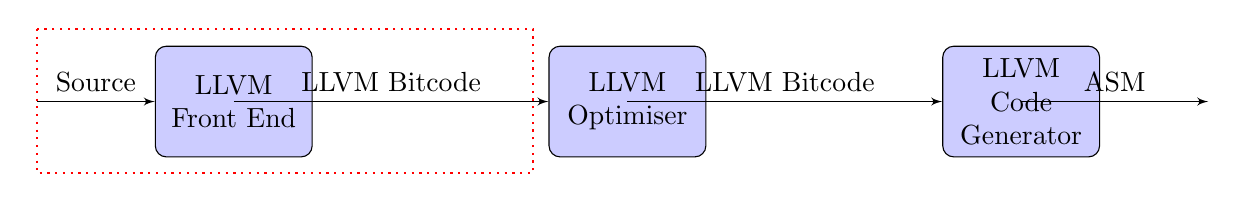
\begin{tikzpicture}[node distance = 5cm, auto]
	\node [] (in) {};
	\node [block, right of=in, node distance=2.5cm] (front) {LLVM Front End};
	\node [block, right of=front] (middle) {LLVM Optimiser};
	\node [block, right of=middle] (end) {LLVM Code Generator};
	\node [right of=end, node distance=2.5cm] (out) {};	
	
	\path [line] (in) |- node [near end, above] {Source} (front);
	\path [line] (front) |- node [near end, above] {LLVM Bitcode} (middle);
	\path [line] (middle) |- node [near end, above] {LLVM Bitcode} (end);	
	\path [line] (end) |- node [near end, above] {ASM} (out);
	
	\draw[thick,red,dotted] ($(in.north)+(0,0.8)$) rectangle ($(middle.south west)-(0.2,0.2)$);
\end{tikzpicture}\\\\
Of this highlighted area there are 3 main parts: the Front-end, the `Middle-end' and the Back-end, the internal workings of which are described below.
\\\\
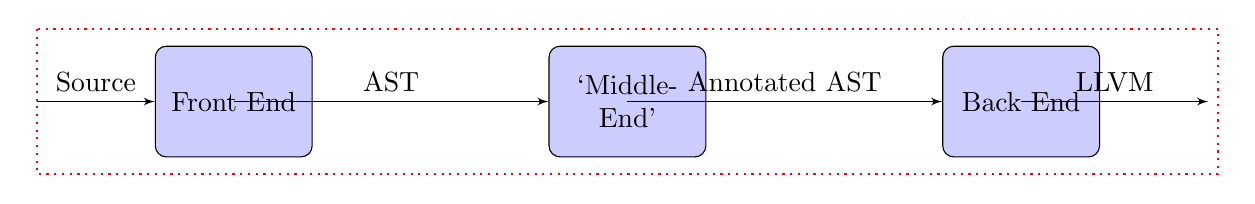
\begin{tikzpicture}[node distance = 5cm, auto]
	\node [] (in) {};
	\node [block, right of=in, node distance=2.5cm] (front) {Front End};
	\node [block, right of=front] (middle) {`Middle-End'};
	\node [block, right of=middle] (end) {Back End};
	\node [right of=end, node distance=2.5cm] (out) {};	
	
	\path [line] (in) |- node [near end, above] {Source} (front);
	\path [line] (front) |- node [near end, above] {AST} (middle);
	\path [line] (middle) |- node [near end, above] {Annotated AST} (end);
	\path [line] (end) |- node [near end, above] {LLVM} (out);
	
	\draw[thick,red,dotted] ($(in.north)+(0,0.8)$) rectangle ($(out.south)-(0,0.8)$);
\end{tikzpicture}\\\\
An overarching design decision was to reduce complexity by \textit{lowering} higher level features of the language to simpler ones, in effect converting to a simpler sublanguage that is easier to generate code for.  The conversion occurs in the `Middle-end' by adding/removing/modifying elements in the AST and results in the `Middle-end' being the most complex part of the compiler, leaving the Back-end fairly simple. Features such as namespaces/using statements, binary operators, template types \& methods and mixins are lowered to just classes, interfaces and regular methods.

\subsection{Front-end}
The Front End performs lexing and parsing, which converts the set of source input files into an \textit{Abstract Syntax Tree} (AST), a set of datastructures representing the program. The lexing and parsing are implemented using fslex and fsyacc respectively, which are versions of the popular ocamllex and ocamlyacc programs ported to \fsharp\cite{fsPowerPack}. 

\subsection{Middle End}
The Middle End performs various transformations on the input data. The raw AST is fed in and various passes happen over it, modifying it slightly each time. The main three operations on the AST are \textit{lowering} of various constructs to simpler ones, \textit{annotation} of the AST with additional data and \textit{checking} that the semantics of the program are correct with respect to the programming language. In order, the major phases that the middle end comprises of are as follows:
\\\\
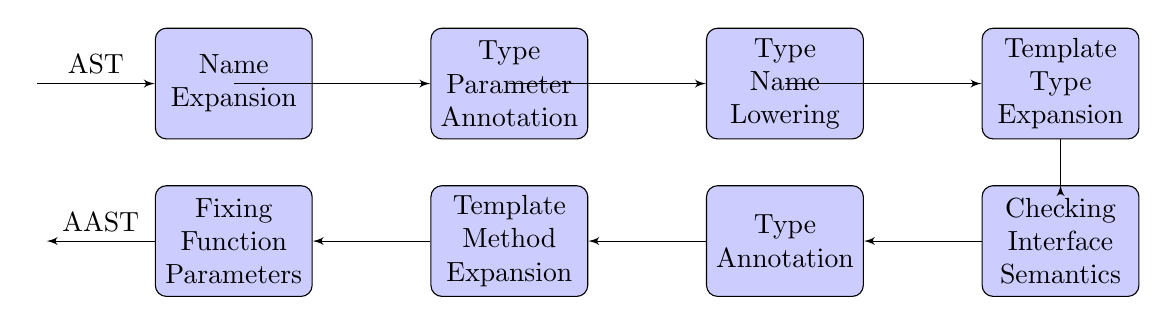
\begin{tikzpicture}[node distance = 3.5cm, auto]
	\node [] (in) {};
	\node [block, right of=in, node distance=2.5cm] (1) {Name Expansion};
	\node [block, right of=1] (2) {Type Parameter Annotation};
	\node [block, right of=2] (3) {Type Name Lowering};
	\node [block, right of=3] (4) {Template Type Expansion};
	\node [block, below of=4, node distance=2cm] (5) {Checking Interface Semantics};
	\node [block, left of=5] (6) {Type Annotation};
	\node [block, left of=6] (7) {Template Method Expansion};
	\node [block, left of=7] (8) {Fixing Function Parameters};
	\node [left of=8, node distance=2.5cm] (out) {};	
	
	\path [line] (in) |- node [near end, above] {AST} (1);
	\foreach \x/\y in {1/2,2/3,3/4} {
		\path [line] (\x) |- (\y);
	}
	\path [line] (4.south) |- (5.north);
	\foreach \x/\y in {5/6,6/7,7/8} {
		\path [line] (\x.west) |- (\y.east);
	}
	\path [line] (8.west) |- node [near end, above] {AAST} (out);
\end{tikzpicture}
\begin{enumerate}
	\item{\textbf{Name Expansion.} Namespaces are removed by adding the namespace to the beginning of the class' name; class \bcode{C} in namespace \bcode{Foo::Bar} becomes class \bcode{Foo::Bar::C}.}
	\item{\textbf{Type Parameter Annotation.} The parser does not know which type names inside a template are type parameters; this process finds uses of type parameters and marks them as such.}
	\item{\textbf{Type Name Lowering.} Types in method signatures are stored as text (e.g. \bcode{Int32}) by the parser; these are resolved to the correct full qualified type in the correct namespace such as \bcode{System::Int32}.}
	\item{\textbf{Template Type Expansion.} Templates are expanded when they are used; a template \bcode{Tem`[A,B]} used as \bcode{Tem`[Int32,Bool]} is expanded out to a new non-template class \bcode{Tem[Int32,Bool]}.}
	\item{\textbf{Checking Interface Semantics.} Checks are performed on the interface inheritance hierarchy; for example, there should be no loops and interface methods should be implemented in classes.}
	\item{\textbf{Type Annotation.} Recursively determining the type for every expression in the program. For example, in the expression \bcode{1 < 2}, \bcode{1} and \bcode{2} both have type \bcode{Int32} and since \bcode{Int32.<(Int32,Int32):Bool} the entire expression has type \bcode{Bool}. This is also where constructs like binary operators are lowered to simple static calls and calls are annotated as static, instance or virtual.}
	\item{\textbf{Fixing Function Parameters.} Instance methods have an implicit \bcode{this} parameter which is used to represent the state of the object the method is being called on. In \plname code, this parameter is not found in instance method definitions but the code generator must know about it, so a \bcode{this} parameter is added in for each1 instance method.}
\end{enumerate}

\subsection{Back End}
The Back End is entirely dedicated to code generation and the production of LLVM assembly code. The llvm-fs project\cite{llvm-fs} is a set of bindings to the LLVM C API from \fsharp that allows the user to build up LLVM assembly language programmatically and also provides some limited form of validation and error checking. Almost all of the section \ref{sec:Implementation} is dedicated to a detailed description of code generation.

\subsection{Testing}
As each feature was written for the compiler, multiple tests were created to check that the correct semantics were being implemented by the compiler. A testing script was written in python that took input file(s) like the one below, extracted the result from between the \bcode{/*[[[} and \bcode{]]]*/}, ran the code and checked to see if the results matched.
\\
\begin{minipage}{0.6\textwidth}
\begin{sooplisting}
class Program {
	static fac(n: Int32): Int32 {
		if (n <= 1)
			return 1;
		return n * fac(n - 1);
	}

	public static main() {
		Console.println(fac(6));
	}
}

/*[[[
720

]]]*/
\end{sooplisting}
\end{minipage}
\begin{minipage}{0.4\textwidth}
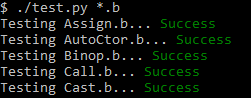
\includegraphics[width=5cm]{test_run}
\end{minipage}
A webapp was also created that allows the user to see the data structures at each stage of the compiler and easily make changes to the test code to quickly track down and find the source of bugs. It also provided a variety of LLVM based debugging and validation info.
\\\\
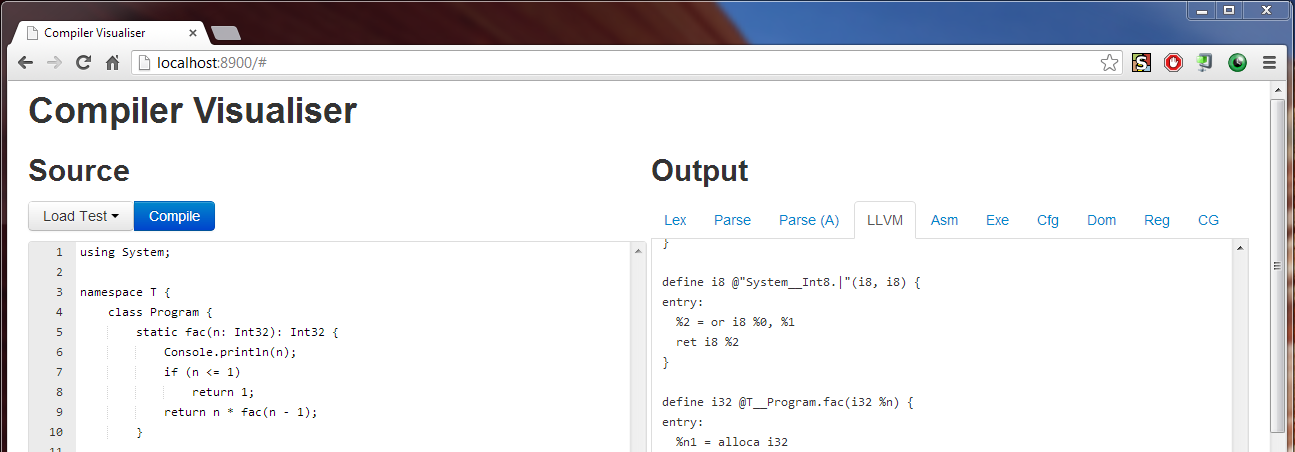
\includegraphics[width=\textwidth]{webapp}

\subsection{LLVM}
LLVM is a compiler infrastructure that takes a platform independent intermediary representation (IR) of a program and compiles it to the appropriate assembly language of a large number of supported back-ends. It has a large portfolio of optimisations that are performed upon the IR enabling the creation of extremely fast and efficient code and has been hugely popular, with front-ends existing for many languages including Haskell, C, C++, Java bytecode, Python, Ruby, GLSL, and OpenCL. The \plname compiler leverages LLVM's features such as it's strong low level type system to compile \plname{} programs to native code with very fast execution speeds.

\subsubsection{LLVM Intermediary Language}
LLVM IR aims to be a ``universal IR'' by providing a set of low level types and operations that every high level language can be mapped to. A summary of the important points of it's syntax and semantics follows but a full explanation of all it's features is avaliable via the LLVM Language Reference\cite{LLVMLangRef}.

\subsubsection{LLVM IR Types}

LLVM IR provides the following primitive types:
\begin{itemize}
	\item{Integer Types: \bcode{i1,i8,i16,i32,i64} where $n$ in \code{i$n$} is the size in bits.}
	\item{Floating Point Types: \bcode{half,float,double} of sizes 16, 32 and 64 bits.}
	\item{Void Type: \bcode{void} representing ``no value''.}
\end{itemize}
From these the following derived types are produced:
\begin{itemize}
	\item{Pointer Type: \bcode{T*} (for type $T$) is a reference a memory location containing a $T$.}
	\item{Structure Type: \bcode{\{ T1,$\dots$,Tn \}} (for types $T1,\dots,Tn$) is a collection of data members in memory.}
	\item{Function Type: \bcode{Tr (T1,$\dots$,Tn)} is a function taking $T1,\dots,Tn$ and returning $Tr$.}
\end{itemize}
The set of all types is the closure of the the above rules. Some rules have been omitted for simplicity.

\subsubsection{LLVM IR Values}
LLVM expressions are in Single Static Assignment (SSA) form - this means that each variable is assigned to exactly once. Expressions take the form \bcode{\%name = op value1, value2, $\dots$, valueN}. Example arithmetic instructions are: \bcode{add,sub,div,mul,$\dots$} and so \bcode{\%0 = add i32 3, i32 \%a} will assign the result of adding $3$ and \bcode{\%a} to \bcode{\%0}. \bcode{load} and \bcode{store} operations read and write from memory, \bcode{alloca} allocates memory on the stack and \bcode{br} is used to provide (un)conditional jumps.


\pagebreak
\section{Implementation}
\label{sec:Implementation}
This sections details the implementation of the major features of the \plname language, showing the LLVM code that is produced from \plname programs and discussing the other implementation options and why they were not selected.

\subsection{Lexing and Parsing}
The Lexing stage takes a set of input files and \textit{tokenises} them, transforming strings of text into tokens that are passed onto the Parsing stage. The Parser takes the tokens and using a grammar converts these to an Abstract Syntax Tree (AST) that represents all the program structures. The position of each fragment of code in the file is passed on in the tokens and is used later to provide useful error messages describing where in the input file the error occurred.

\subsubsection{Abstract Syntax Tree}
The AST has 4 main components: \bcode{NamespaceDecl}s, \bcode{ClassDecl}s, \bcode{InterfaceDecl}s and \bcode{Expr}s. Each of these immutable types has a ``annotation type'' that acts as a wrapper and allows data to be attached to the declaration after it has been created by the parser. The annotation type for a particular declaration has an ``\bcode{A}'' on the end such as \bcode{NamespaceDeclA} and \bcode{ClassDeclA}. The definition of the AST is shown below.

\begin{fslisting}
type NamespaceDecl =
    | Class of Name * Visibility * IsStruct * (*interfaces*) list<PType> * list<ClassDeclA>
    | Interface of Name * Visibility * (*interfaces*) list<PType> * list<InterfaceDeclA>
   
type InterfaceDecl =
    | InterfaceProc of Name * list<Param> * (*returnType*) PType ref

type ClassDecl =
    | ClassVar  of Name * Visibility * IsStatic * PType ref * ExprA
    | ClassProc of Name * Visibility * IsStatic * list<Param> ref * (*returnType*) PType ref * (*body*) ExprA

type Expr =
    | ConstInt of (*size*) int * (*value*) int64
    | ConstBool of bool
    | Var of string
    | VarStatic of PType ref
    | Dot of ExprA * string
    | Binop of string * ExprA * ExprA
    | Cast of PType ref * ExprA
    | Call of ExprA * list<ExprA>
    | Assign of ExprA * ExprA
    | DeclVar of string * (*Assign*) ExprA
    | Return of ExprA
    | ReturnVoid
    | If of ExprA * ExprA * ExprA
    | While of ExprA * ExprA
    | For of ExprA * ExprA * ExprA * ExprA
    | Seq of ExprA ref * ExprA ref
    | Nop
\end{fslisting}

\subsection{Basic Statements}
\subsubsection{If Statements}
Take the following simple if statement; if b is true print 1 else print 2:
\begin{sooplisting}
public static main() {
	val b = true;
	if (b)
		Console.println(1);
	else
		Console.println(2);
}
\end{sooplisting}
This method becomes the following LLVM code:\\
\begin{minipage}{0.62\textwidth}
\begin{llvmlisting}
define void @T__Program.main() {
entry:
  ; val b = true;
  %b = alloca i1
  store i1 true, i1* %b
  %b1 = load i1* %b
  ; if(b)
  br i1 %b1, label %ifThen, label %ifElse

ifThen:
  ; Console.println(1);
  call void @System__Console.println(i32 1)
  br label %ifCont

ifElse:
  ; Console.println(2);
  call void @System__Console.println(i32 2)
  br label %ifCont

ifCont:
  ret void
}
\end{llvmlisting}
\end{minipage}
\begin{minipage}{0.38\textwidth}
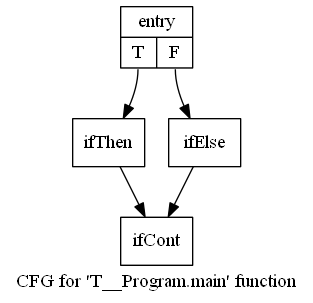
\includegraphics[width=6cm]{if_cfg_small}
\end{minipage}

\subsubsection{While Loops}
Taking following simple while loop, which prints out the numbers from 6 down to 0:
\begin{sooplisting}
public static main() {
	var i = 6;
	while (i >= 0) {
		Console.println(i);
		i = i - 1;
	}
}
\end{sooplisting}
This method becomes the following LLVM code:
\\\\
\begin{minipage}{0.62\textwidth}
\begin{llvmlisting}
define void @T__Program.main() {
entry:
  ; var i = 6
  %i = alloca i32
  store i32 6, i32* %i
  br label %whileTest

whileTest:
  ; while (i >= 6)
  %i1 = load i32* %i
  %0 = call i1 @"System__Int32.>="(i32 %i1, i32 0)
  br i1 %0, label %whileBody, label %whileCont

whileBody:
  ; Console.println(i);
  %i2 = load i32* %i
  call void @System__Console.println(i32 %i2)
  ; i = i - 1;
  %i3 = load i32* %i
  %1 = call i32 @System__Int32.-(i32 %i3, i32 1)
  store i32 %1, i32* %i
  br label %whileTest

whileCont:
  ret void
}
\end{llvmlisting}
\end{minipage}
\begin{minipage}{0.38\textwidth}
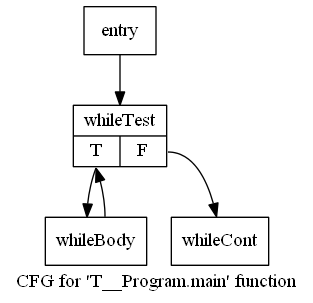
\includegraphics[width=6cm]{while_cfg_small}
\end{minipage}
A \bcode{for} loop is very similar and has 

\subsection{Layout of Class Types}
A class of the form:
\begin{sooplisting}
class Foo {
	private var x1: Type1;
	private var x2: Type2;
	// ...
	public var xN: TypeN;
	
	public static foo(a: Int32):Int32 { return a; }
	public bar(a: Int32):Int32 { return a; }
}
\end{sooplisting}
Is changed into the following LLVM bitcode. An aggregate type with enough space for all the instance variables is created. Variables and method parameters have space on the stack allocated to them by the \bcode{alloca} command, then are read and written by the \bcode{load} and \bcode{store} commands respectively. Extraneous \bcode{store}s and \bcode{load}s that can be safely removed are removed by the LLVM optimiser. A \bcode{ctor} method is also created that allocates space on the heap and returns a constructed object.
\begin{llvmlisting}
%K__Foo = type { %VTable*, Type1, Type2, ..., TypeN }

; Has a 'this' parameter as it is an instance method
define i32 @K__Foo.bar(%K__Foo* %this, i32 %a) {
entry:
  ; Allocate space and store the 'this' parameter in it
  %this1 = alloca %K__Foo*
  store %K__Foo* %this, %K__Foo** %this1
  ; Allocate space and store the 'a' parameter in it
  %a2 = alloca i32
  store i32 %a, i32* %a2
  ; Load the value of 'a'
  %a3 = load i32* %a2
  ; Return 'a'
  ret i32 %a3
}

; Does not have a 'this' parameter as it is a static method
define i32 @K__Foo.foo(i32 %a) {
entry:
  %a1 = alloca i32
  store i32 %a, i32* %a1
  %a2 = load i32* %a1
  ret i32 %a2
}

define %K__Foo* @"K__Foo+ctor"() {
entry:
  ; Allocate space on the heap - the subexpression in @malloc(-) is a way to find the size of a struct
  %malloc = call i8* @malloc(i32 ptrtoint (%K__Foo* getelementptr (%K__Foo* null, i32 1) to i32))
  %0 = bitcast i8* %malloc to %K__Foo*
  ; Store the object's VTable; more on this in a later section
  %1 = getelementptr inbounds %K__Foo* %0, i32 0, i32 0
  store %VTable* @VTable___K__Foo, %VTable** %1
  ret %K__Foo* %0
}
\end{llvmlisting}

\subsection{Method Overloading/Selection}
\label{sec:methodOverloadSelection}
Method overloading allows multiple methods to have the same name but accept different arguments. The example below shows method overloading on \bcode{test}.
\begin{sooplisting}
interface Bar {}
class BarImpl() : Bar {}

interface Foo {}
class FooImpl() : Foo {}

class Test {
	static test(b: Bar, x: Foo) {} // 1
	static test(b: Bar, x: FooImpl) {} // 2
	static test(b: BarImpl, x: Foo) {} // 3		
}
\end{sooplisting}
If we define the following variables:
\begin{sooplisting}
var bi = BarImpl.new();
var b  = [Bar] bi;
var fi = FooImpl.new();
var f  = [Foo] fi;
\end{sooplisting}
Then the following calls will be matched with the methods described in the comments.
\begin{sooplisting}
test(b, fi);  // test(Bar,FooImpl)
test(b, f);   // test(Bar,Foo)
test(bi, fi); // Cannot choose between test(Bar, FooImpl) and test(BarImpl, Foo)
\end{sooplisting}
The algorithm to determine which overload to use from a set of possible methods $M$, a name $n$ and a list of argument types $T$ is as follows:
\begin{enumerate}
	\item{Make a set $M'$ which contains the methods from $M$ that have the name $n$ and have the correct number of parameters $length(T)$.}
	\item{For each $m \in M'$: take $m$'s list of parameter types $P$ (in the form \bcode{n($p_1,p_2,\dots,p_{|P|}$)}) and perform the following sum:
		\begin{enumerate}
			\item{For each argument type $t \in T$ and parameter type $p \in P$, if $t$ equals $p$ score $2$, else if $t$ is a subtype of $p$ score 1, else score $-\infty$.}
			\item{Sum all of the scores to get an overall score $s$}
		\end{enumerate}
	}
	\item{Return highest scoring method $m$; if there is more than one with the same highest score, or they are all $-\infty$, error.}
\end{enumerate}

\subsection{Interfaces and VTables}
Multiple checks are performed on interfaces -- the strongly connected components of the interface inheritance hierarchy are found using Tarjan's algorithm to see if there are any cycles which would cause an unresolvable loop to be created. There are also checks to see whether each type implementing the interface implements all the interface's methods.

Interfaces allow the mechanism of dynamic dispatch which is implemented using Virtual Method Tables (VTables). Conceptually, a VTable is an array of function pointers that that each point to a particular type's implementation of a certain set of methods. At runtime, the correct implementation of a method can be determined from the type of the object.

\subsubsection{VTable Structure}
\label{sec:VTableStructure}
To explain the VTable creation process, let's look at a concrete example of a \plname program:
\begin{sooplisting}
interface Vehicle {
	drive();
	getNumberOfWheels():Int8;
}

interface Flying {
	getAltitude():Int32;
}

class Car : Vehicle {
	public drive() { }
	public getNumberOfWheels():Int8 { return 4B; }
}

class Airplane : Vehicle, Flying {
	public drive() { }
	public getNumberOfWheels():Int8 { return 2B; }
	public getAltitude():Int32 { return 42000; }
}
\end{sooplisting}
The process advances as follows:
\begin{enumerate}
	\item{
		Each interface method is given a unique id.
		\begin{center}
		\begin{tabular}{ | c | c | }
		\hline
		\textbf{Interface Method} & \textbf{ID} \\ \hline
		\bcode{Flying.getAltitude():Int32} & 0 \\ \hline
		\bcode{Vehicle.drive()} & 1 \\ \hline
		\bcode{Vehicle.getNumberOfWheels():Int8} & 2 \\ \hline
		\end{tabular}
		\end{center}			
	}
	\item{
		A \bcode{VTable} type is created - it is a struct containing a function pointer for each interface method (ordered according to their id). The first \bcode{\%Interface*} parameter is the ``this'' parameter that passes the calling object to the method.
		\begin{llvmlisting}
%VTable = type { i32 (%Interface*)*, void (%Interface*)*, i8 (%Interface*)* }
		\end{llvmlisting}
	}
	\item{
		The concrete types are then constructed, each with a pointer to it's VTable as the first field.
		\begin{llvmlisting}
%T__Airplane = type { %VTable* }
%T__Car = type { %VTable* }
%Interface = type { %VTable* }
		\end{llvmlisting}
	}
	\item{
		For each type $T$ an instance of the \bcode{VTable} is instantiated - for each interface method that $T$ implements, a function pointer to $T$'s method implementation is put into the \bcode{VTable}.
		\begin{llvmlisting}
@VTable___T__Airplane = global %VTable {
	i32 (%Interface*)* @"T::Airplane.getAltitude+Stub", 
	void (%Interface*)* @"T::Airplane.drive+Stub", 
	i8 (%Interface*)* @"T::Airplane.getNumberOfWheels+Stub" }
@VTable___T__Car = global %VTable { 
	i32 (%Interface*)* null,
	void (%Interface*)* @"T::Car.drive+Stub",
	i8 (%Interface*)* @"T::Car.getNumberOfWheels+Stub" }
		\end{llvmlisting}
	}
	\item {
		Stub methods are created into order to keep using (and so take advantage of) LLVM's strong type system. They cast the generic \bcode{\%Interface} type to the concrete type and call the original method. There is no overhead from these extra function calls as they be inlined by the LLVM optimiser.
		\begin{llvmlisting}
define i32 @"T::Airplane.getAltitude+Stub"(%Interface* %this) {
entry:
  %0 = bitcast %Interface* %this to %T__Airplane*
  %1 = call i32 @T__Airplane.getAltitude(%T__Airplane* %0)
  ret i32 %1
}
		\end{llvmlisting}
	}
\end{enumerate}
Graphically, the layout of the LLVM types can be presented as:\\
% http://tex.stackexchange.com/questions/40128/creating-process-table-figure-in-tikz
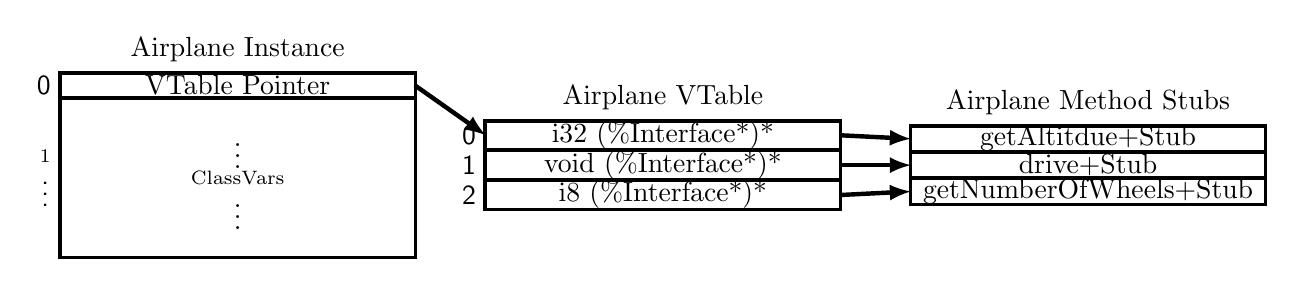
\begin{tikzpicture}
\matrix (class) at (0,0) [table matrix,label={[align=center]90:{Airplane Instance}}]
{
VTable Pointer\\
|[minimum height=2cm]| $\substack{\vdots\\ \mathrm{Class Vars}\\ \vdots}$\\
};

\matrix (vtable) at (5.4,0) [table matrix,label={[align=center]90:{Airplane VTable}}]
{
i32 (\%Interface*)*\\
void (\%Interface*)*\\
i8 (\%Interface*)*\\
};

\matrix (stubs) at (10.8,0) [table matrix,label={[align=center]90:{Airplane Method Stubs}}]
{
getAltitdue+Stub\\
drive+Stub\\
getNumberOfWheels+Stub\\
};

\foreach \x/\y in {1/0,2/$\substack{1\\ \vdots}$} {
	\node[anchor=east] at (class-\x-1.west) {\textsf{\y}};
}
\foreach \x/\y in {1/0,2/1,3/2} {
	\node[anchor=east] at (vtable-\x-1.west) {\textsf{\y}};
}
\draw[black,-latex,ultra thick] (class-1-1.east) -- (vtable-1-1.west);
\foreach \x in {1,2,3} {
	\draw[black,-latex,ultra thick] (vtable-\x-1.east) -- (stubs-\x-1.west);
}
%\draw[black,-latex,ultra thick] (vtable-2-1.east) -- (stubs-1-1.west);
%\draw[black,-latex,ultra thick] (vtable-3-1.east) -- (stubs-2-1.west);
\end{tikzpicture}

\subsubsection{Virtual Method Call}
Following on from the previous example, let's see what would happen if we were to perform a virtual method call on the \bcode{drive} method of a \bcode{Vehicle}:
\begin{sooplisting}
var v = [Vehicle] Airplane.new();
v.drive();
\end{sooplisting}
Focusing on the \bcode{v.drive()} statement, assuming \bcode{\%v} is a pointer to the value of \bcode{v}:
\begin{enumerate}
	\item{
		Load the reference to \bcode{v} into \bcode{\%v1}.
		\begin{llvmlisting}
%v1 = load %Interface** %v
		\end{llvmlisting}
	}
	\item{
		Load the pointer to \bcode{Car}'s 0th element (its VTable) into \bcode{\%3}.
		\begin{llvmlisting}
%2 = getelementptr inbounds %Interface* %v1, i32 0, i32 0
%3 = load %VTable** %2
		\end{llvmlisting}
	}
	\item{
		Load the VTable's 1st element (its function pointer for \bcode{Vehicle.drive}) into \bcode{\%5}.
		\begin{llvmlisting}
%4 = getelementptr inbounds %VTable* %3, i32 0, i32 1
%5 = load void (%Interface*)** %4
		\end{llvmlisting}
	}
	\item{
		Call the function, passing the reference to \bcode{v} as the \bcode{this} parameter.
		\begin{llvmlisting}
call void %5(%Interface* %v1)
		\end{llvmlisting}
	}
\end{enumerate}

\subsubsection{Other Approaches Considered}
Another way to layout the VTables was considered but not implemented because of performance concerns; instead of having a single VTable pointer attached to each object instance as described above, each object would have many VTable pointers, one pointer for each interface that it implemented. Each VTable would have an ``offset'' field that is the position in the instance type of the VTable pointer.\\\\
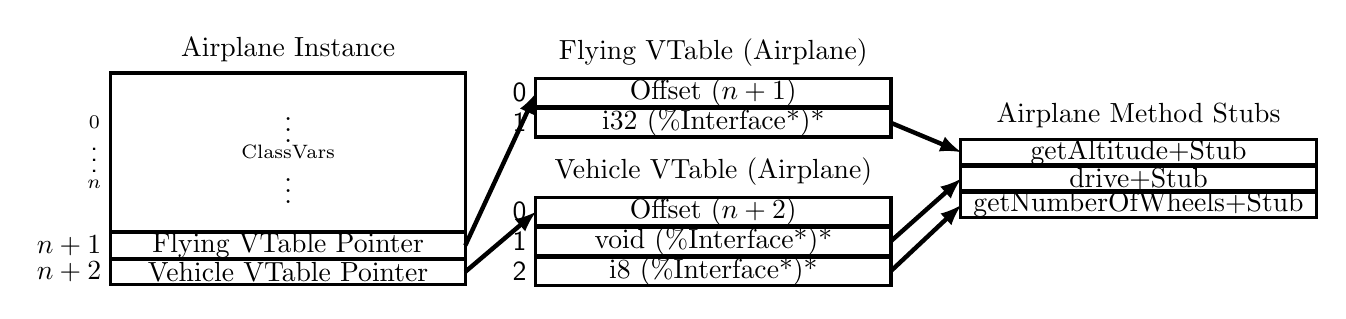
\begin{tikzpicture}
\matrix (class) at (0,0) [table matrix,label={[align=center]90:{Airplane Instance}}]
{
|[minimum height=2cm]| $\substack{\vdots\\ \mathrm{Class Vars}\\ \vdots}$\\
Flying VTable Pointer\\
Vehicle VTable Pointer\\
};

\matrix (vtableFlying) at (5.4,0.9) [table matrix,label={[align=center]90:{Flying VTable (Airplane)}}]
{
Offset ($n+1$)\\
i32 (\%Interface*)*\\
};

\matrix (vtableVehicle) at (5.4,-0.8) [table matrix,label={[align=center]90:{Vehicle VTable (Airplane)}}]
{
Offset ($n+2$)\\
void (\%Interface*)*\\
i8 (\%Interface*)*\\
};

\matrix (stubs) at (10.8,0) [table matrix,label={[align=center]90:{Airplane Method Stubs}}]
{
getAltitude+Stub\\
drive+Stub\\
getNumberOfWheels+Stub\\
};

\foreach \x/\y in {1/$\substack{0\\ \vdots \\n}$,2/$n+1$,3/$n+2$} {
	\node[anchor=east] at (class-\x-1.west) {\textsf{\y}};
}
\foreach \x/\y in {1/0,2/1} {
	\node[anchor=east] at (vtableFlying-\x-1.west) {\textsf{\y}};
}
\foreach \x/\y in {1/0,2/1,3/2} {
	\node[anchor=east] at (vtableVehicle-\x-1.west) {\textsf{\y}};
}

\draw[black,-latex,ultra thick] (class-2-1.east) -- (vtableFlying-1-1.west);
\draw[black,-latex,ultra thick] (class-3-1.east) -- (vtableVehicle-1-1.west);
\draw[black,-latex,ultra thick] (vtableFlying-2-1.east) -- (stubs-1-1.west);
\foreach \x/\y in {2/2,3/3} {
	\draw[black,-latex,ultra thick] (vtableVehicle-\x-1.east) -- (stubs-\y-1.west);
}
%
\end{tikzpicture}
When a object is casted to an interface (say \bcode{Vehicle}), rather than just changing the type of the object and leaving the pointer to the object as is, the pointer to the object would be changed to point to the appropriate VTable Pointer (at offset $n+2$).
\\\\
When performing a virtual call (on say \bcode{v.drive()} where \bcode{v} is of type \bcode{Vehicle}), the pointer to \bcode{v} is pointing to the `Vehicle VTable Pointer' -- we follow this to reach the `Vehicle VTable' and the offset. The \bcode{drive+Stub} method is accessed by loading the appropriate offset (1) in the `Vehicle VTable' and a pointer to the start of the object is reconstructed by subtracting the offset from the pointer to \bcode{v}. The stub method is then called using the reconstructed pointer for the `this' argument.
\\\\
However, the problems with this approach are numerous:
\begin{itemize}
	\item{It reduces the total memory requirement of the VTables by ensuring that VTable entries only exist if they are going to be used (in the implemented version, \bcode{Car} has a VTable entry for \bcode{Flying.getAltitude} even though it does not implement \bcode{Flying}) but increases the size of each object instance in proportion to the number of interfaces it implements. Since there is only one set of VTable(s) created for each object but possibly thousands or millions of objects, this approach is likely to require much more memory.}
	\item{It is more complex, requiring object pointers to be pointing to the right part of the interior of the object; casts are no longer trivial and an offset must be used to calculate the object starting location when performing virtual calls.}
	\item{Introduces \textit{interior pointers} to the implementation, which slows down most garbage collectors.}
	\item{Has no speed benefit over the implemented version.}
\end{itemize}

\subsection{Binary Operators}
Binary operators are defined as \bcode{public static} methods that use symbols instead of names and have precisely two parameters. In the \textit{Binop Lowering Phase}, a list $L$ of every binary operator is compiled by searching each class for all the methods that fit this definition. For each \bcode{Binop (name, left, right)} expression in the AST, the best overload $m$ from $L$ fitting the \bcode{name} and types of \bcode{left} and \bcode{right} is selected and the \bcode{Binop} expression is replaced by a static call to $m$ (as described in section \ref{sec:methodOverloadSelection}). For example, using the following binary operator definition: 
\begin{sooplisting}
class Operators {
	public static **(a: Int32, b: Int32): Int32 {
		return a * a + b * b;	
	}
}
\end{sooplisting}
The AST of the following expression:
\begin{sooplisting}
1 ** 3; // Binop (Var "**", ConstInt (32, 1), ConstInt (32, 3))
\end{sooplisting}
Will be changed into an AST that would be created from the following equivalent code:
\begin{sooplisting}
Operators.**(1, 3);
// Call (Dot (VarStatic "Operators", "**")), [ConstInt (32, 1), ConstInt (32, 1)]
\end{sooplisting}

\subsubsection{Precedence}
The binary operator precedence is defined similar to FSharp -- the first character of the operator determines its precedence from the table below. When an operator of precedence level $p$ is lexed, a token of the form \bcode{BINOP$p$} is created; in fsyacc (the parsing stage) the tokens \bcode{BINOP$p$} for $p=1,2,\dots,6$ have their precedence ordered by the \bcode{\%left} instruction.
\begin{center}
\begin{tabular}{ | c | c | }
\hline
\textbf{Operator Character} & \textbf{Precedence} \\ \hline
* / & 6 \\ \hline
\% & 5 \\ \hline
+ $-$ & 4 \\ \hline
= < > & 3 \\ \hline
? ! & 2 \\ \hline
\& & 1 \\ \hline
| & 0 \\ \hline
\end{tabular}
\end{center}
Special treatment is given to the \bcode{\&\&} and \bcode{||} operators so that they short circuit. 

%\subsection{Arrays}
%$a[i]$ gets changed to a.indexer(i)\\
%$a[x_1][x_2]\dots[x_n] = v$ is lowered to \code{a.indexer($x_1$).indexer($x_2$)}$\dots$\code{.indexer($x_n$,$v$)}

\subsection{Templates}
Template in \plname are implemented in a similar way to templates in \cpp; they are form of typesafe macro expansion that creates \textit{concrete} expanded implementations of template types when provided with a list of type parameters.

\subsubsection{Syntax}
\label{sec:TemplateSyntax}
The syntax for templates in \plname differs from the most other implementations -- the form \bcode{TypeName<T1,T2,$\dots$,Tn>} is used by \csharp, Java, \cpp and many others but leads to ambiguities when lexing and parsing. When used with the standard binary operators \bcode{<}, \bcode{>} and function calls using parentheses and commas, the expression \bcode{foo(TypeName<A,B>.bar)} cannot be parsed with an LR(1) parser. Ambiguity arises when the parsing automaton reaches the comma - without looking ahead at least 3 tokens (and seeing the full stop) and it cannot decide whether the statment should be parsed as \bcode{foo(TypeName is less than A,...)} or \bcode{foo(TypeName with generic parameters A,...)}. Lexing is also a problem as the operator \bcode{>}\bcode{>} is often used as the right bitshift operator which can cause issues in types with nested template parameters like \bcode{Box<Box<Int32>}\bcode{>}.

\plname avoids these problems by using the unambiguous form \bcode{TypeName`[T1,T2,$\dots$,Tn]} where $T1 \dots Tn$ are the \textit{type parameters}.
\begin{sooplisting}
class Box`[T] {
	private var item: T;
	
	public static new(item: T):Box`[T] {
		var b = ctor();
		b.item = item;
		return b;
	}
	
	public getItem():T { return item; }

	public static main() {
        Box`[Int32].new(3);
        Box`[Bool].new(true);
    }
}
\end{sooplisting}
As you can see from how the above example is transformed into LLVM, two new types \bcode{\%K\_\_Box[System\_\_Bool]} and \bcode{\%K\_\_Box[System\_\_Int32} are created each with their own \bcode{getItem()} method.
\begin{llvmlisting}
%"K__Box[System__Bool]" = type { %VTable*, i1 }
%"K__Box[System__Int32]" = type { %VTable*, i32 }

define i1 @"K__Box[System__Bool].getItem"(%"K__Box[System__Bool]"* %this) {
entry:
  %this1 = alloca %"K__Box[System__Bool]"*
  store %"K__Box[System__Bool]"* %this, %"K__Box[System__Bool]"** %this1
  ; return item;
  %0 = load %"K__Box[System__Bool]"** %this1
  %1 = getelementptr inbounds %"K__Box[System__Bool]"* %0, i32 0, i32 1
  %2 = load i1* %1
  ret i1 %2
}

define i32 @"K__Box[System__Int32].getItem"(%"K__Box[System__Int32]"* %this) {
entry:
  %this1 = alloca %"K__Box[System__Int32]"*
  store %"K__Box[System__Int32]"* %this, %"K__Box[System__Int32]"** %this1
  ; return item;
  %0 = load %"K__Box[System__Int32]"** %this1
  %1 = getelementptr inbounds %"K__Box[System__Int32]"* %0, i32 0, i32 1
  %2 = load i32* %1
  ret i32 %2
}


\end{llvmlisting}

\subsubsection{Template Expansion}
Template expansion takes place in two stages: in the first stage, called \textit{Template Type Expansion}, parametrised data types are expanded; in the second stage, called \textit{Template Method Expansion} parametrised methods are expanded. 

\paragraph{Template Type Expansion}
A depth first search is performed on the AST with the non-template data types as roots. The program descends the AST and for each template declaration of a template type (say \bcode{Tem`[Foo,Bar]}) it checks if it has already been found, if not it clones the template type replacing the type parameters with the appropriate concrete types. The listing below shows the possible places that a template can be instantiated once all constructs have been lowered to the base classes/structs and interfaces.
\begin{sooplisting}
class Class`[...] : ~~IFace1`[...]~~,...,~~IFaceN`[...]~~ {

	public method`[...](t1: ~~Type1`[...]~~, ..., tN: ~~TypeN`[...]~~):~~Type`[...]~~ {
		[~~CastType[...]~~] castExpr;
		var foo = ~~VarStaticType[...]~~.dotName;
	}	
	private var variable: ~~Type`[...]~~;
}

interface IFace`[...] : ~~IFace1`[...]~~,...,~~IFaceN`[...]~~ {
	public method`[...](t1: ~~Type1`[...]~~, ..., tN: ~~TypeN`[...]~~):~~Type`[...]~~;
}
\end{sooplisting}

\paragraph{Template Method Expansion}
Methods cannot be expanded until the \textit{Type Annotation Phase} as the types of the calling arguments must be known in order to select the correct overload. For example, on a class \bcode{Foo} there may exist static methods \bcode{bar`[T](a:Bool, b:T)} and \bcode{bar`[T](a:Int32, b:T)} -- which template method is expanded for a call of \bcode{Foo.bar`[Int32](v,0)} depends on the type of \bcode{v}. Similarly, for \bcode{a.foo`[Type]()} the type of \bcode{a} must be known to determine which datatype to expand \bcode{foo} in.\\\\
For example, take the following piece of code that causes template method expansion for a static call:
\begin{sooplisting}
class Program {
	public static id`[A](a: A, b: Int32):A { return a; }
	public static id`[A](a: A, b: Bool):A  { return a; }
	public static id`[A,B](a: A, a:B):A    { return a; }

	public static main() {
		Program.id`[Int32](3,true);
	}
}
\end{sooplisting}
The algorithm to expand the templates proceeds as follows, with the example in brackets:
\begin{enumerate}
	\item{In an expression (\bcode{main()}) a parametrised static call $c$ (\bcode{Program.id`[Int32](3,true)}) is found}.
	\item{The set of methods signatures $M$ in the target type $T$ (\bcode{Program}) that are static and have the same name (\bcode{id}), number of type parameters (1) and number of formal parameters (2) as $c$ is constructed ($\{\bcode{id`[A](A,Int32)}, \bcode{id`[A](A,Bool)}\}$).}
	\item{Template expansion is performed on each signature $m \in M$ in isolation, returning a set of expanded methods signatures $M'$ ($\{\bcode{id(Int32,Int32)}, \bcode{id(Int32,Bool)}\}$).}
	\item{Out of $M'$ the appropriate expanded overload $m'$ is selected (\bcode{id(Int32,Bool)} using the process described in section \ref{sec:methodOverloadSelection}).}
	\item{The method that expanded out to have signature $m'$ is fully expanded and added to $T$.}
\end{enumerate}
Instance calls cause expansion in the same way only with $T$ differing and performing the search for instance rather than static methods. 


\subsubsection{Other Approaches Considered}
\label{sec:TemplateOtherApproaches}
Another approach was considered but again dropped for performance reasons, although it does have some benefits over the implemented version. Rather than using \cpp like template expansions where whole new types are created for each different set of type parameters, something similar to Java's implementation of generics could have been developed instead. With this approach, only one version of code would be needed; a `generic' version of the class would be created using \textit{type erasure} by changing all instances of type parameters in the class to be an \bcode{\%Interface*} type. This would mean that any type could use the outputted LLVM as only virtual calls could happen, which is in effect just dealing with various pointers.
\\\\
Benefits:
\begin{itemize}
	\item{Only one implementation per set of type parameters needs to be created -- avoids massive code expansion, increased compile times, extremely long type signatures.}
\end{itemize}
Problems:
\begin{itemize}
	\item{Since the only operations on the type parameter types are virtual calls, value types like \bcode{Int*} and \bcode{Bool} could not be used, or would have to be boxed, which would ruin performance.}
	\item{In the template implementation, operations on a type parameter that is not an interface will use regular calls and not virtual calls; for this implementation, virtual calls are always used and each call imposes a significant two memory load tax.}
	\item{The way binary operators have been implemented is not compatible with this implementation; the types of the operands must be known at compile time which is not so in a generic class.}	
	\item{In the template implementation, once the templates have been expanded to their concrete types there are no more templates; the rest of the compiler, especially the code generation stage, need not do anything special for these expanded types. With this implementation the rest of the compiler would have to be `generic-aware', significantly increasing the complexity.}
\end{itemize}


\section{Review and Future Work}
\subsection{Problems and Possible Improvements}
\paragraph{Garbage Collection.}
Currently there is no garbage collection -- objects have space allocated on the heap with \bcode{malloc} and are never \bcode{free}d. Each program slowly leaks memory until it runs out and then crashes. This could be very easily fixed by using the Boehm-Demers-Weiser conservative garbage collector, which would only require linking an extra library with the output of the LLVM code generator and changing all calls to \bcode{malloc} to \bcode{GC\_MALLOC}.

\paragraph{Bindings to LLVM.}
The llvm-fs bindings used to generate the LLVM code are somewhat incomplete and buggy; a lot of the time on the project was spent either improving or adding to the llvm-fs project in order to iron out bugs or add desperately needed features. The LLVM project itself must bare some of the blame, as the C API that the llvm-fs bindings depend on\footnote{And the OCaml, Python, Haskell, etc bindings} is incomplete and undocumented compared to the provided \cpp framework. Debugging was also made difficult by use of barebones \cpp assertion errors used by the LLVM shared library and problems with native code interop from managed \fsharp code. This was partly mitigated by the design of the compiler -- passing off complexity from the Back-end to the `Middle-end' by reducing to a simpler language meant less work was needed on the code generator. Work to make the LLVM C API and llvm-fs bindings feature complete would make a many more features possible and greatly speed up the development process.

\paragraph{Heavy use of mutability.}
The ``Middle-end'' of the compiler heavily uses \textit{annotation} by attaching pieces of information to the AST. Whilst this reduces amount of code required to perform the operations (as the AST does not need to be continually rewritten) the use of this mutable information can allow subtle bugs to slip in, especially in operations such as template expansion where making multiple new copies of existing AST sections can lead to references being accidentally shared between copies or the AST section not being copied properly. This would be easier to reason about if the structures were less mutable, so a future refactoring of the compiler could be to make more of the data structures in the AST immutable.

\paragraph{Templates.}
Heavy use of templates leads to an explosion in the size of the output code -- for every unique set of type parameters used on a template type a completely new type is created. This also leads to long type signatures such as: 
\begin{llvmlisting}
%G__Foo[G__Bar[G__Foo[G__Bar[System__Int32]]]] ; Foo`[Bar`[Foo`[Bar`[Int32]]]]
\end{llvmlisting}
Which can confuse debugging when there is type name of this size on every line. Also, compilation speeds suffer with templates as many new types need to be created and have various operations performed on them. \cpp, which has a similar implementation of templates, also has this problem and there does not seem to be a way around it other than trying to make the operations the compiler performs faster, or using a different method to achieve parametric polymorphism as described in section \ref{sec:TemplateOtherApproaches}.

\paragraph{Exception/Error Handling.}
\plname currently has no exceptions or any form of error handling -- only \bcode{Application.crash()} is provided by the standard library as a reliable way to stop the program executing. In it's present state, the language could be used to return `success' or `failure' objects to enable some kind of error handling but this is not included in the standard library. LLVM has an exceptions API that could be leveraged to provide exceptions for \plname, however significant work to enable this in llvm-fs would be required.

\paragraph{Standard Library.}
The standard library is rather lacking, providing only integer, boolean, floating point and array types, as well as a class \bcode{Console} that can print and read data to \bcode{stdout} and from \bcode{stdin}. It does not have the collection types and others operations that would be expected in the standard library; future work would include expanding it's functionality until it is useful.

\subsection{Conclusion}
The aims of the project were to create a compiler for a statically typed, memory safe object oriented programming language that had features to help with code reuse, mutability and null safety as well as provided parametric polymorphism and being reasonably fast. The compiler fulfils all of these aims.
The language is object oriented -- it fits the requirements set out in section \ref{sec:OOPIntro}: polymorphism and subtyping are provided by interfaces, encapsulation is enabled by the use of visibility modifiers like \bcode{private} and behavioural reuse is can be achieved through use of mixins. It is statically typed as we cannot modify the operations on types (field and methods) after compilation and memory safe as the user is unable to access raw memory and pointers and can only deal with references. Mixins provide code reuse, mutability is discouraged as the default variable declaration, \bcode{val}, is immutable and null safety is provided by not allowing null references. Finally, parametric polymorphism is provided in the form of templates.

%\section{Code}
%The code for the project is too large to be printed here but can be accessed at: ...

%At the end it contained approximately:
%\begin{itemize}
%	\item{\textbf{\fsharp:} 3720 SLOC}
%\end{itemize}

\printbibliography

\end{document}





















































